\documentclass[twoside]{book}

% Packages required by doxygen
\usepackage{fixltx2e}
\usepackage{calc}
\usepackage{doxygen}
\usepackage[export]{adjustbox} % also loads graphicx
\usepackage{graphicx}
\usepackage[utf8]{inputenc}
\usepackage{makeidx}
\usepackage{multicol}
\usepackage{multirow}
\PassOptionsToPackage{warn}{textcomp}
\usepackage{textcomp}
\usepackage[nointegrals]{wasysym}
\usepackage[table]{xcolor}

% Font selection
\usepackage[T1]{fontenc}
\usepackage[scaled=.90]{helvet}
\usepackage{courier}
\usepackage{amssymb}
\usepackage{sectsty}
\renewcommand{\familydefault}{\sfdefault}
\allsectionsfont{%
  \fontseries{bc}\selectfont%
  \color{darkgray}%
}
\renewcommand{\DoxyLabelFont}{%
  \fontseries{bc}\selectfont%
  \color{darkgray}%
}
\newcommand{\+}{\discretionary{\mbox{\scriptsize$\hookleftarrow$}}{}{}}

% Page & text layout
\usepackage{geometry}
\geometry{%
  a4paper,%
  top=2.5cm,%
  bottom=2.5cm,%
  left=2.5cm,%
  right=2.5cm%
}
\tolerance=750
\hfuzz=15pt
\hbadness=750
\setlength{\emergencystretch}{15pt}
\setlength{\parindent}{0cm}
\setlength{\parskip}{3ex plus 2ex minus 2ex}
\makeatletter
\renewcommand{\paragraph}{%
  \@startsection{paragraph}{4}{0ex}{-1.0ex}{1.0ex}{%
    \normalfont\normalsize\bfseries\SS@parafont%
  }%
}
\renewcommand{\subparagraph}{%
  \@startsection{subparagraph}{5}{0ex}{-1.0ex}{1.0ex}{%
    \normalfont\normalsize\bfseries\SS@subparafont%
  }%
}
\makeatother

% Headers & footers
\usepackage{fancyhdr}
\pagestyle{fancyplain}
\fancyhead[LE]{\fancyplain{}{\bfseries\thepage}}
\fancyhead[CE]{\fancyplain{}{}}
\fancyhead[RE]{\fancyplain{}{\bfseries\leftmark}}
\fancyhead[LO]{\fancyplain{}{\bfseries\rightmark}}
\fancyhead[CO]{\fancyplain{}{}}
\fancyhead[RO]{\fancyplain{}{\bfseries\thepage}}
\fancyfoot[LE]{\fancyplain{}{}}
\fancyfoot[CE]{\fancyplain{}{}}
\fancyfoot[RE]{\fancyplain{}{\bfseries\scriptsize Generated by Doxygen }}
\fancyfoot[LO]{\fancyplain{}{\bfseries\scriptsize Generated by Doxygen }}
\fancyfoot[CO]{\fancyplain{}{}}
\fancyfoot[RO]{\fancyplain{}{}}
\renewcommand{\footrulewidth}{0.4pt}
\renewcommand{\chaptermark}[1]{%
  \markboth{#1}{}%
}
\renewcommand{\sectionmark}[1]{%
  \markright{\thesection\ #1}%
}

% Indices & bibliography
\usepackage{natbib}
\usepackage[titles]{tocloft}
\setcounter{tocdepth}{3}
\setcounter{secnumdepth}{5}
\makeindex

% Hyperlinks (required, but should be loaded last)
\usepackage{ifpdf}
\ifpdf
  \usepackage[pdftex,pagebackref=true]{hyperref}
\else
  \usepackage[ps2pdf,pagebackref=true]{hyperref}
\fi
\hypersetup{%
  colorlinks=true,%
  linkcolor=blue,%
  citecolor=blue,%
  unicode%
}

% Custom commands
\newcommand{\clearemptydoublepage}{%
  \newpage{\pagestyle{empty}\cleardoublepage}%
}

\usepackage{caption}
\captionsetup{labelsep=space,justification=centering,font={bf},singlelinecheck=off,skip=4pt,position=top}

%===== C O N T E N T S =====

\begin{document}

% Titlepage & ToC
\hypersetup{pageanchor=false,
             bookmarksnumbered=true,
             pdfencoding=unicode
            }
\pagenumbering{roman}
\begin{titlepage}
\vspace*{7cm}
\begin{center}%
{\Large Reference Manual\\[1ex]\large .. }\\
\vspace*{1cm}
{\large Generated by Doxygen 1.8.11}\\
\end{center}
\end{titlepage}
\clearemptydoublepage
\tableofcontents
\clearemptydoublepage
\pagenumbering{arabic}
\hypersetup{pageanchor=true}

%--- Begin generated contents ---
\chapter{Class Index}
\section{Class List}
Here are the classes, structs, unions and interfaces with brief descriptions\+:\begin{DoxyCompactList}
\item\contentsline{section}{\hyperlink{classclass__handle}{class\+\_\+handle$<$ base $>$} }{\pageref{classclass__handle}}{}
\item\contentsline{section}{\hyperlink{classRMF_1_1Node}{R\+M\+F\+::\+Node} \\*\hyperlink{classRMF_1_1Node}{Node} is the building blocks of modules logic }{\pageref{classRMF_1_1Node}}{}
\item\contentsline{section}{\hyperlink{classRMF_1_1Internal_1_1Route__}{R\+M\+F\+::\+Internal\+::\+Route\+\_\+} \\*Internal class to represent connections between topics provided and listened internally by nodes and in global space of a Master }{\pageref{classRMF_1_1Internal_1_1Route__}}{}
\end{DoxyCompactList}

\chapter{Class Documentation}
\hypertarget{classclass__handle}{}\section{class\+\_\+handle$<$ base $>$ Class Template Reference}
\label{classclass__handle}\index{class\+\_\+handle$<$ base $>$@{class\+\_\+handle$<$ base $>$}}
\subsection*{Public Member Functions}
\begin{DoxyCompactItemize}
\item 
{\bfseries class\+\_\+handle} (base $\ast$ptr)\hypertarget{classclass__handle_ac68e361cb6bce4d42148e8f7f9a81f81}{}\label{classclass__handle_ac68e361cb6bce4d42148e8f7f9a81f81}

\item 
bool {\bfseries is\+Valid} ()\hypertarget{classclass__handle_af6132f4dcc9eec3ebcfe6ccb1cea857f}{}\label{classclass__handle_af6132f4dcc9eec3ebcfe6ccb1cea857f}

\item 
base $\ast$ {\bfseries ptr} ()\hypertarget{classclass__handle_a770ba105e71c5b331ce2144fd570a603}{}\label{classclass__handle_a770ba105e71c5b331ce2144fd570a603}

\end{DoxyCompactItemize}


The documentation for this class was generated from the following file\+:\begin{DoxyCompactItemize}
\item 
interface/matlab/tools/class\+\_\+handle/class\+\_\+handle.\+hpp\end{DoxyCompactItemize}

\hypertarget{classRMF_1_1Node}{}\section{R\+MF\+:\+:Node Class Reference}
\label{classRMF_1_1Node}\index{R\+M\+F\+::\+Node@{R\+M\+F\+::\+Node}}


\hyperlink{classRMF_1_1Node}{Node} is the building blocks of modules logic.  




{\ttfamily \#include $<$Node.\+hpp$>$}

\subsection*{Public Member Functions}
\begin{DoxyCompactItemize}
\item 
virtual void {\bfseries update} ()\hypertarget{classRMF_1_1Node_a26d161c468575d913c9c62d7297035b9}{}\label{classRMF_1_1Node_a26d161c468575d913c9c62d7297035b9}

\end{DoxyCompactItemize}


\subsection{Detailed Description}
\hyperlink{classRMF_1_1Node}{Node} is the building blocks of modules logic. 

They contain all the process and communicate with each other using Topics. You can define a \hyperlink{classRMF_1_1Node}{Node} by inheriting from this class.

\begin{DoxyAuthor}{Author}
\href{mailto:a.sharpasand@mrl-spl.ir}{\tt Mohammad Ali Sharpasand} 
\end{DoxyAuthor}
\begin{DoxyVersion}{Version}
0.\+0.\+1 
\end{DoxyVersion}
\begin{DoxyCopyright}{Copyright}
M\+IT License. 
\end{DoxyCopyright}


The documentation for this class was generated from the following file\+:\begin{DoxyCompactItemize}
\item 
include/Node.\+hpp\end{DoxyCompactItemize}

\hypertarget{classRMF_1_1Internal_1_1Route__}{}\section{R\+MF\+:\+:Internal\+:\+:Route\+\_\+ Class Reference}
\label{classRMF_1_1Internal_1_1Route__}\index{R\+M\+F\+::\+Internal\+::\+Route\+\_\+@{R\+M\+F\+::\+Internal\+::\+Route\+\_\+}}


Internal class to represent connections between topics provided and listened internally by nodes and in global space of a Master.  




{\ttfamily \#include $<$Master.\+hpp$>$}



Collaboration diagram for R\+MF\+:\+:Internal\+:\+:Route\+\_\+\+:\nopagebreak
\begin{figure}[H]
\begin{center}
\leavevmode
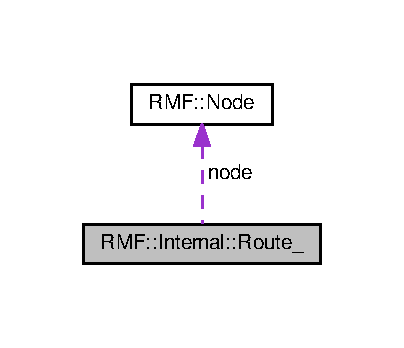
\includegraphics[width=194pt]{classRMF_1_1Internal_1_1Route____coll__graph}
\end{center}
\end{figure}
\subsection*{Public Attributes}
\begin{DoxyCompactItemize}
\item 
\hyperlink{classRMF_1_1Node}{Node} {\bfseries node}\hypertarget{classRMF_1_1Internal_1_1Route___a42ac220416ed21a3a72aea631439b644}{}\label{classRMF_1_1Internal_1_1Route___a42ac220416ed21a3a72aea631439b644}

\item 
std\+::string {\bfseries internal\+Topic}\hypertarget{classRMF_1_1Internal_1_1Route___a6e8e519abbfbd0e267945ec2e691fef9}{}\label{classRMF_1_1Internal_1_1Route___a6e8e519abbfbd0e267945ec2e691fef9}

\item 
std\+::string {\bfseries public\+Topic}\hypertarget{classRMF_1_1Internal_1_1Route___ac7ac0545070d02e23e32fc4ef3e85992}{}\label{classRMF_1_1Internal_1_1Route___ac7ac0545070d02e23e32fc4ef3e85992}

\end{DoxyCompactItemize}


\subsection{Detailed Description}
Internal class to represent connections between topics provided and listened internally by nodes and in global space of a Master. 

\begin{DoxyAuthor}{Author}
\href{mailto:a.sharpasand@mrl-spl.ir}{\tt Mohammad Ali Sharpasand} 
\end{DoxyAuthor}
\begin{DoxyVersion}{Version}
0.\+0.\+1 
\end{DoxyVersion}
\begin{DoxyCopyright}{Copyright}
M\+IT License. 
\end{DoxyCopyright}


The documentation for this class was generated from the following files\+:\begin{DoxyCompactItemize}
\item 
include/Master.\+hpp\item 
include/Route.\+hpp\end{DoxyCompactItemize}

%--- End generated contents ---

% Index
\backmatter
\newpage
\phantomsection
\clearemptydoublepage
\addcontentsline{toc}{chapter}{Index}
\printindex

\end{document}
